%%%%%%%%%%%%%%%%%%%%%%%%%%%%%%%%%%%%%%%%%

%\title{Title page with logo}
%----------------------------------------------------------------------------------------
%	PACKAGES AND OTHER DOCUMENT CONFIGURATIONS
%----------------------------------------------------------------------------------------

\documentclass[11pt]{article}
\usepackage[portuguese]{babel}
\usepackage[utf8x]{inputenc}
\usepackage{amsmath}
\usepackage{amssymb}
\usepackage{graphicx}
\usepackage{natbib}
\usepackage{cite} 
\usepackage{float}
\usepackage{calrsfs}
\usepackage[a4paper,left=2.5cm,right=2cm,top=2.5cm, bottom=2cm]{geometry}
\usepackage{verbatim}
\usepackage{bigints}
\usepackage{booktabs}
\usepackage[table]{xcolor}
\usepackage{siunitx}

\begin{document}

\begin{titlepage}

\newcommand{\HRule}{\rule{\linewidth}{0.5mm}} % Defines a new command for the horizontal lines, change thickness here

\center % Center everything on the page
 
%----------------------------------------------------------------------------------------
%	HEADING SECTIONS
%----------------------------------------------------------------------------------------

\textsc{\LARGE Universidade Federal de Alagoas}\\[1.5cm] % Name of your university/college
\textsc{\Large Instituto de Computação (IC)}\\[0.5cm] % Major heading such as course name
\textsc{\large Laboratório de Computação Científica e Análise Numérica (LaCCAN)}\\[3.5cm] % Minor heading such as course title

%----------------------------------------------------------------------------------------
%	TITLE SECTION
%----------------------------------------------------------------------------------------

\HRule \\[0.4cm]
{ \LARGE \bfseries Fluxograma de Execução da Rotina de Estimação}\\[0.4cm] 
\HRule \\[2.5cm]
 
%----------------------------------------------------------------------------------------
%	AUTHOR SECTION
%----------------------------------------------------------------------------------------

\begin{minipage}{0.4\textwidth}
\begin{flushleft} \large
\emph{Autor:}\\
Marcos G. S. do Nascimento % Your name
\end{flushleft}
\end{minipage}
~
\begin{minipage}{0.4\textwidth}
\begin{flushright} \large
\emph{Orientador:} \\
Alejandro C. Frery  % Supervisor's Name
\end{flushright}
\end{minipage}\\[8cm]

% If you don't want a supervisor, uncomment the two lines below and remove the section above
%\Large \emph{Author:}\\
%John \textsc{Smith}\\[3cm] % Your name

%----------------------------------------------------------------------------------------
%	DATE SECTION
%----------------------------------------------------------------------------------------

{\large 25/02/2019}\\[2cm] % Date, change the \today to a set date if you want to be precise

%----------------------------------------------------------------------------------------
%	LOGO SECTION
%----------------------------------------------------------------------------------------

% \includegraphics{logo.png}\\[1cm] % Include a department/university logo - this will require the graphicx package
 
%----------------------------------------------------------------------------------------

\vfill % Fill the rest of the page with whitespace

\end{titlepage}


\section{Introdução}
O presente relatório visa abordar o funcionamento geral da rotina de estimação que encapsula os algoritmos de estimação implementados e tem autonomia para tomar alguma decisão e executar alguma das técnicas desenvolvidas, diante de cada situação prevista. 

Com base nos experimentos de Monte Carlo que foram realizados foi possível fazer uma avaliação geral da qualidade de cada técnica implementada analisando o desempenho de cada uma delas em diferentes cenários considerando diferentes números de \textit{Looks}, diferentes graus de textura da imagem - homogênea, heterogênea ou extremamente heterogênea - e diferentes tamanhos de amostra. O funcionamento de tal rotina de estimação foi pensado com base na análise de estudos feitos na literatura e, sobretudo, com base nos experimentos realizados.

Na seção seguinte temos o fluxograma do funcionamento geral da rotina de estimação, bem como algumas explicações e diretrizes que foram tomadas para a sua construção. 

\section{Fluxograma de Execução da Rotina de Estimação}

Abaixo encontra-se o fluxograma de execução propriamente dito. O seguinte raciocínio foi levado em consideração para a construção desse fluxograma:
\begin{itemize}
    \item No início temos a interação com o usuário onde o mesmo tem a opção de escolher um algoritmo em especial para executar a estimação ou então não indicar opção alguma e deixar o sistema escolher a mais apropriada para cada caso.
    \item Se foi escolhido um algoritmo específico, o sistema vai tentar executar esse algoritmo e, se não ocorrer falhas, retorna o estimador calculado. Se houver falha, o sistema também saberá como agir verificando o tamanho da amostra e seguindo adiante até a execução de outro estimador.
    \item Se não foi escolhido um algoritmo específico ou se houver falha no passo anterior, há a verificação do tamanho da amostra da entrada. Se $n < 200$, parte-se para o método de Log-Cumulantes que se mostrou apropriado para trabalhar com amostras pequenas. O sistema vai tentar executar esse método e, se não houver falhas, retorna o estimador calculado. Se houver falha, parte-se para a verificação do número de \textit{Looks} e o sistema segue adiante até a execução de outro estimador.
    \item Se o tamanho da amostra for maior ou igual que 200 ($n >= 200$) ou se houver falha no passo anterior, há a verificação do número de \textit{Looks}. No caso em que $Looks <= 5$ executa-se a estimação por Máxima Verossimilhança que forneceu resultados bem precisos nesse caso e o estimador é calculado, se não houver falhas. Se falhar, parte-se para a verificação da textura da região.
    \item No caso em que temos $Looks > 5$ ou se houver falha no passo anterior, faz-se a verificação da textura por meio do parâmetro $\alpha$. A estimação por Distâncias Estocásticas utiliza métodos de minimização que são mais estáveis e possuem menor erro nos casos em que temos um número grande de \textit{Looks} e valores próximos de zero do parâmetro $\alpha$ que correspondem a regiões extremamente rugosas da imagem, conforme aborda \citet{Cassetti2013} em seu trabalho. Assim, o sistema vai tentar executar esse algoritmo de Distâncias Estocásticas e exibir o resultado. Se houver falhas, parte-se para o método dos Momentos. 
    \item Por sua vez, o método dos momentos vai ser executado no caso em que o parâmetro $\alpha <= -3$ ou se houver falha no passo anterior e, caso não ocorra falhas, o resultado será exibido. Se houver falhas, executa-se a estimação pelo algoritmo de Máxima Verossimilhança (foi o que apresentou os melhores resultados no geral) e exibe-se o resultado. Se esse algoritmo falhar, exibe-se a mensagem de erro para o usuário e solicita-se para o mesmo tentar novamente com dados válidos.
    
\end{itemize}
\begin{figure}[H]
     \centering
     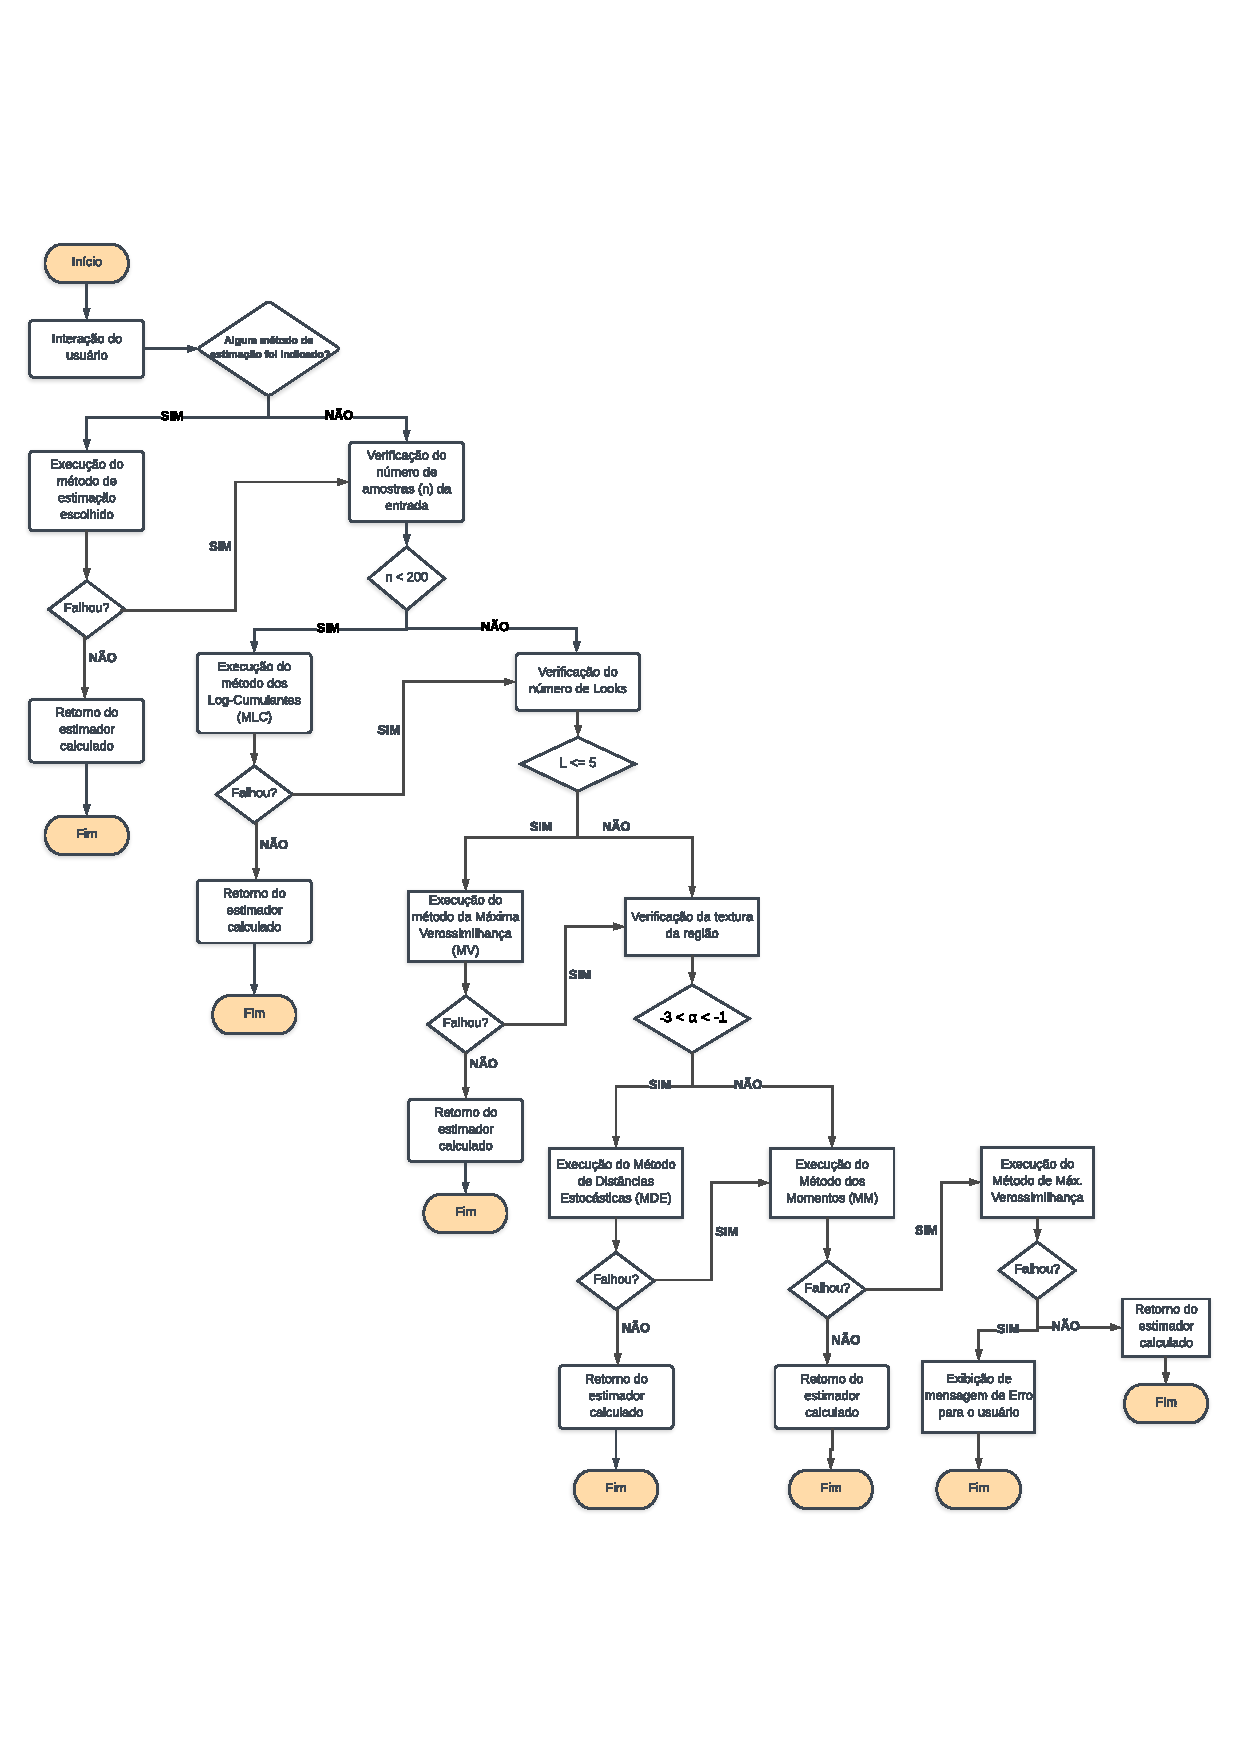
\includegraphics[scale=0.80]{FluxogramaDeExecucao-A4.pdf}
     \caption{Fluxograma de execução da rotina de estimação}
     \label{fig1}
\end{figure}


\newpage
\bibliographystyle{agsm}
%\bibliographystyle{unsrt}
\bibliography{../../../Bibliography/references}
%\bibliography{references}


\end{document}